% qudisclose: coordinated vulnerability disclosure, agent to agent
% Build: tectonic qudisclose.tex
% Layout and palette follow the Quome paper style (ink, teal, violet).
\documentclass[11pt]{article}
\usepackage[margin=1.05in]{geometry}
\usepackage{graphicx}
\usepackage{booktabs}
\usepackage{array}
\usepackage{xcolor}
\usepackage{microtype}
\usepackage{enumitem}
\usepackage{amsmath}
\usepackage[hidelinks]{hyperref}
\usepackage{caption}
\usepackage{tikz}
\usetikzlibrary{arrows.meta, positioning}
\captionsetup{font=small,labelfont=bf}

\definecolor{ink}{HTML}{15161d}
\definecolor{teal}{HTML}{12857a}
\definecolor{violet}{HTML}{a45cf0}
\definecolor{tealtint}{HTML}{dcf5f1}
\definecolor{lavender}{HTML}{f3f1fb}
\definecolor{muted}{HTML}{6b6f80}

\setlist{nosep}
\renewcommand{\topfraction}{0.92}\renewcommand{\bottomfraction}{0.6}\renewcommand{\textfraction}{0.06}\renewcommand{\floatpagefraction}{0.75}
\setcounter{topnumber}{3}\setcounter{totalnumber}{4}
\newcommand{\qud}{\texttt{qudisclose}}
\newcommand{\vsla}{\textsc{vsla}}
\newcommand{\lvl}[1]{\textbf{L#1}}
\newcommand{\code}[1]{\texttt{\small #1}}

\newcommand{\glance}[3]{%
  \begin{tikzpicture}[baseline=(current bounding box.north)]
    \node[draw=#1, line width=0.9pt, rounded corners=9pt, fill=#1!5, inner xsep=10pt, inner ysep=9pt, text width=0.275\textwidth, minimum height=2.6cm, align=left, anchor=north west]
      {{\scriptsize\sffamily\bfseries\color{#1}\MakeUppercase{#2}}\\[0.3em]{\footnotesize #3}};
  \end{tikzpicture}}

\begin{document}

% ------------------------------------------------------------------ cover page
\thispagestyle{empty}
\noindent
\begin{minipage}[c]{0.72\textwidth}
  \raggedright\includegraphics[height=1.05cm]{figs/quome.png}
\end{minipage}\hfill
\begin{minipage}[c]{0.25\textwidth}
  \raggedleft\itshape\large November 2026
\end{minipage}

\vspace{1.4em}
\noindent{\fontsize{28}{32}\selectfont\bfseries\color{ink}qudisclose\par}
\vspace{0.2em}
\noindent{\fontsize{19}{23}\selectfont\bfseries\color{ink}Coordinated Vulnerability Disclosure,\\Agent to Agent\par}
\vspace{0.5em}
\noindent
\begin{tikzpicture}\shade[left color=teal, right color=violet] (0,0) rectangle (3.4cm,0.11cm);\end{tikzpicture}
\vspace{0.4em}

\noindent{\large\itshape\color{ink} A machine-to-machine intake, an agent team, and the controls that make it safe.\par}
\vspace{1.0em}

\noindent\begin{minipage}{0.6\textwidth}
  {\large Jim Schwoebel\textsuperscript{1,2}}\\[0.2em]
  {\small \textsuperscript{1}\,Quome, Inc.\quad \textsuperscript{2}\,Advanced AI Society\quad\texttt{jim@quome.com}}
\end{minipage}\hfill
\begin{minipage}{0.36\textwidth}\raggedleft
  {\small working draft v0.1}\\[0.2em]
  {\small\texttt{github.com/quome-cloud/qudisclose}}
\end{minipage}

\vspace{1.0em}
\noindent{\color{teal}\rule{\textwidth}{0.4pt}}
\vspace{0.6em}

\noindent{\itshape Coordinated disclosure was built for people with inboxes. The finders are increasingly not
people, and a maintainer who answers at human speed has made the latency of the process the vulnerability
window. What does the receiving side look like when it is a machine too, and what has to be true before a
maintainer lets it act?\par}

\vspace{0.9em}
\begin{center}
  \includegraphics[width=0.68\linewidth]{figs/fig-flow.pdf}
\end{center}
\vspace{0.4em}

\noindent
\glance{teal}{Intake and pipeline}{A signed, scoped MCP intake; six agent roles from triage to postmortem; an SLO clock on every case; a short embargo that ends when the fix publishes.}\hfill
\glance{violet}{Verified by code}{A report is believed when the platform's own re-run of a failing test fails by assertion; a patch when it passes in a clean worktree and a reviewer that never saw the patcher's reasoning approves.}\hfill
\glance{ink}{Controls, each with a test}{Per-message signatures, one scope per tool, leased credentials, a signed audit chain, sandboxed execution and \vsla{} trust levels, mapped to the NSA's MCP guidance.}

\newpage

% ------------------------------------------------------------------ abstract
\thispagestyle{empty}
\noindent{\footnotesize\sffamily\bfseries\color{teal}\MakeUppercase{Abstract}}\par
\vspace{0.3em}
\noindent
\begin{tikzpicture}\shade[left color=teal, right color=violet] (0,0) rectangle (2.2cm,0.09cm);\end{tikzpicture}
\vspace{0.8em}

\noindent\begin{minipage}{\textwidth}
{\linespread{1.06}\selectfont
Coordinated vulnerability disclosure (CVD) assumes a person at each end: a researcher who writes to a security
address and a maintainer who reads it, triages in a thread, fixes by hand and publishes weeks later. Scanners,
fuzzers and research agents now produce findings at machine speed and then wait on that process. We describe
\qud{}, an open-source system that is the receiving half of the loop for an open-source project. A reporter's
agent submits a finding over the Model Context Protocol (MCP) with a bearer token and an Ed25519-signed
envelope; feeds from GitHub, Dependabot, OSV and signed webhooks arrive through the same intake. An orchestrator
acknowledges at once and drives six agent roles (triage, reproducer, patcher, reviewer, release, postmortem)
against a service-level clock. The design rule is that no stage is believed on a model's word: the orchestrator
re-runs the reproducing test and requires an assertion failure, applies each patch in a clean worktree and runs
the suite, and gives the reviewer the report, the diff and the test output but never the patcher's reasoning.
The system opens a pull request and a draft advisory and stops; a person merges. Around the pipeline sit the
controls that the NSA's 2026 guidance on MCP asks for, each with a test: per-message integrity and replay
protection, least privilege per tool, short-lived credential leases, distinct non-human identities, a
hash-chained signed audit log, tool-catalog pinning, untrusted-input handling and sandboxed execution. \qud{}
also implements \vsla{}, the graded trust framework for machine disclosures, in both roles: it attests the cases
it verifies and it re-executes, receipts and countersigns the statements reporters submit. We report what is
implemented and tested (127 tests, including the failure paths), one offline end-to-end run, and, as plainly,
what is not yet shown: the live model path has been exercised against a recording client and one self-hosted
model run, not against a population of real reports, and we make no claim about fix quality or time-to-fix on
real projects.
\par}
\end{minipage}

\vspace{1.0em}
\noindent{\color{teal}\rule{\textwidth}{0.4pt}}
\setcounter{page}{1}

% ------------------------------------------------------------------ 1
\section{Introduction}

The standard account of coordinated disclosure~\cite{iso29147,iso30111,certcvd} is a conversation between
people. A researcher reports privately; the maintainer acknowledges, triages, fixes and publishes; an embargo,
conventionally ninety days~\cite{p0}, bounds how long the researcher waits. Each step is paced by a person's
attention. For a solo or small open-source maintainer that pacing is the exposure: the bug is known to at least
one outside party from the first email, and the window stays open until someone has time.

Two things have changed. The finders are increasingly automated, so reports arrive faster than a person can
read them, and a growing share of them are fluent, plausible and wrong~\cite{slopsurvey,herodevs}. And the tools
to answer automatically now exist: a model can read a report, write a test, and propose a patch. The obvious
response, pointing an agent at the security inbox, is unsafe in exactly the ways that matter. The report is
attacker-controlled text. The proof of concept is attacker-controlled code. The agent holds credentials that can
write to the repository. And a model that says a patch works has said nothing a maintainer can rely on.

\qud{} is our attempt to build the receiving side properly. Its contributions are:

\begin{itemize}[leftmargin=1.4em, itemsep=0.25em]
  \item \textbf{A machine-to-machine intake} (Section~\ref{sec:intake}): reports arrive as MCP tool calls from
  pinned non-human identities, signed per message, scoped per tool, idempotent on content, with the project's
  policy published as a resource so a reporter knows the rules before it submits.
  \item \textbf{A pipeline in which code, not the model, decides} (Section~\ref{sec:pipeline}): reproduction,
  patch verification and review are each checked by something the producing agent does not control.
  \item \textbf{A security architecture mapped to published guidance} (Section~\ref{sec:security}): each design
  consideration in the NSA's information sheet on MCP~\cite{nsamcp} corresponds to a class and to a test.
  \item \textbf{An implementation of \vsla{} in both roles} (Section~\ref{sec:vsla}), byte-compatible with the
  reference verifier~\cite{vsla}.
  \item \textbf{A proactive half} (Section~\ref{sec:hunter}): a hunter loop designed to run continuously on a
  self-hosted model and to escalate only what it has reproduced.
\end{itemize}

\noindent We are deliberate about scope. This paper describes a v0.1 system and what its test suite
establishes. It does not report a field study, and Section~\ref{sec:limits} lists what remains unshown.

% ------------------------------------------------------------------ 2
\section{Background}

\paragraph{Coordinated disclosure.} ISO/IEC 29147 and 30111 and the CERT guide~\cite{iso29147,iso30111,certcvd}
define the roles (finder, vendor, coordinator), the phases (report, triage, remediation, publication) and the
expectations (acknowledgement, embargo, credit). None of them assumes a particular transport, and in practice
the transport is email or a web form. Outputs have converged on machine-readable formats, CVSS for
severity~\cite{cvss} and OSV for advisories~\cite{osv}, while inputs have not.

\paragraph{MCP, and the NSA's guidance on it.} The Model Context Protocol gives a model a typed interface to
tools and resources on a server. The NSA's May 2026 information sheet~\cite{nsamcp} treats an MCP deployment as
a continuum in which model, client, server and tools share one effective trust domain, and lists design
considerations rather than a checklist: integrity of each message beyond transport security, least privilege at
the tool boundary, brokered credentials, distinct identities, an audit trail of inputs and outputs, pinned tool
catalogs, tool output treated as untrusted, sandboxed execution, and human review for irreversible actions.
We used that list as the security requirements for \qud{}.

\paragraph{\vsla{}.} A signed message proves who sent a report. It does not prove that the bug is real, that the
named model did the work, or that the account of the work is complete. \vsla{}~\cite{vsla} is a graded
framework, modelled on \textsc{slsa}~\cite{slsa} and carried as in-toto statements~\cite{intoto} in DSSE
envelopes~\cite{dsse}, that answers those questions at four levels (Figure~\ref{fig:ladder}): \lvl{0} no
statement; \lvl{1} a signed statement binding the report to a code revision, a model bill of materials, a
Merkle-rooted transcript~\cite{rfc6962} and a reproduction executed by code; \lvl{2} a platform's own
re-execution, receipt and a countersigned ledger over a floor; \lvl{3} an attested environment. \vsla{} is the
framework; \qud{} is one implementation of it, and this paper is the description of that implementation.

\begin{figure}[t]
  \centering\includegraphics[width=0.92\linewidth]{figs/fig-ladder.pdf}
  \caption{The \vsla{} levels that \qud{} claims as a finder and verifies as a platform.}
  \label{fig:ladder}
\end{figure}

% ------------------------------------------------------------------ 3
\section{Design goals and threat model}
\label{sec:threats}

We set five goals. \textbf{(G1)} Acknowledge immediately and keep a clock on every stage. \textbf{(G2)} Believe
nothing on a model's assertion. \textbf{(G3)} Hold no long-lived authority in any agent's context.
\textbf{(G4)} Leave a record that the agents cannot rewrite. \textbf{(G5)} Keep a person in control of the one
irreversible step, merging, and of any other step the policy names.

The adversaries we design against are these.

\begin{description}[leftmargin=1.4em, labelsep=0.5em, itemsep=0.3em, font=\normalfont\bfseries]
  \item[A malicious or mistaken reporter.] Submits a report whose text tries to instruct the agents, a proof of
  concept that attacks the machine it runs on, a finding that does not exist, a flood of findings, or a replay
  of someone else's.
  \item[A network intermediary.] Alters or replays a tool call in transit, or stands up a look-alike server
  whose tool catalog differs from the one the reporter pinned.
  \item[A compromised or misled agent.] An agent that has been prompt-injected, or is simply wrong, claims a
  reproduction that did not fail, a patch that does not fix, or tries to use a credential for something other
  than its purpose.
  \item[A curious coordinator.] A party with read access who should learn that a fix exists and when, but not
  what the bug is, until publication.
\end{description}

\noindent Out of scope: a compromised host or operator, a malicious maintainer, and the security of the model
provider. \vsla{}'s higher levels speak to some of these; \qud{} at v0.1 does not claim them
(Section~\ref{sec:limits}).

% ------------------------------------------------------------------ 4
\section{The system}

\begin{figure}[t]
\centering
\resizebox{\linewidth}{!}{%
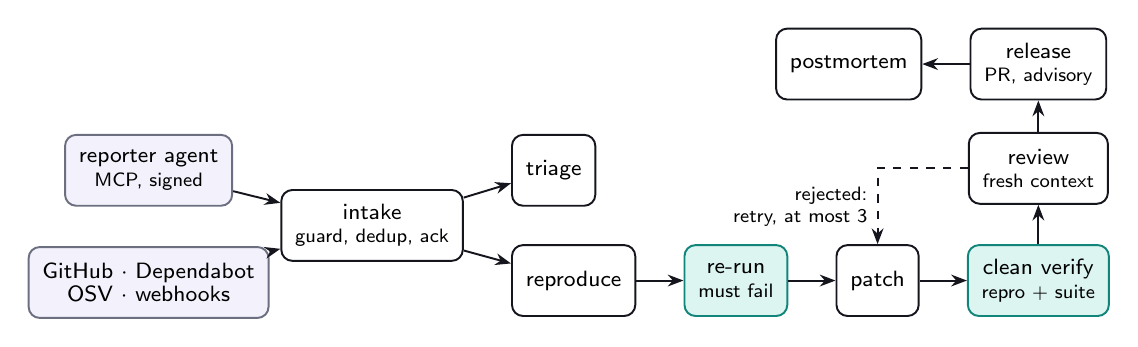
\begin{tikzpicture}[
    node distance=5mm and 6mm, font=\sffamily\footnotesize,
    box/.style={draw=ink, line width=0.7pt, rounded corners=4pt, fill=white, inner sep=5pt, align=center, minimum height=9mm},
    code/.style={box, fill=tealtint, draw=teal},
    src/.style={box, fill=lavender, draw=muted},
    arr/.style={-{Stealth[length=2mm]}, line width=0.7pt, draw=ink}]
  \node[src] (rep) {reporter agent\\[-1pt]{\scriptsize MCP, signed}};
  \node[src, below=of rep] (feeds) {GitHub $\cdot$ Dependabot\\[-1pt]OSV $\cdot$ webhooks};
  \node[box, right=of rep, yshift=-7mm] (intake) {intake\\[-1pt]{\scriptsize guard, dedup, ack}};
  \node[box, right=of intake, yshift=7mm] (triage) {triage};
  \node[box, right=of intake, yshift=-7mm] (repro) {reproduce};
  \node[code, right=of repro] (rerun) {re-run\\[-1pt]{\scriptsize must fail}};
  \node[box, right=of rerun] (patch) {patch};
  \node[code, right=of patch] (verify) {clean verify\\[-1pt]{\scriptsize repro + suite}};
  \node[box, above=of verify] (review) {review\\[-1pt]{\scriptsize fresh context}};
  \node[box, above=of review, yshift=-1mm] (release) {release\\[-1pt]{\scriptsize PR, advisory}};
  \node[box, left=of release] (pm) {postmortem};
  \draw[arr] (rep) -- (intake); \draw[arr] (feeds) -- (intake);
  \draw[arr] (intake) -- (triage); \draw[arr] (intake) -- (repro);
  \draw[arr] (repro) -- (rerun); \draw[arr] (rerun) -- (patch); \draw[arr] (patch) -- (verify);
  \draw[arr] (verify) -- (review); \draw[arr] (review) -- (release); \draw[arr] (release) -- (pm);
  \draw[arr, dashed] (review.west) -| node[pos=0.75, left, align=right, font=\sffamily\scriptsize]{rejected:\\retry, at most 3} (patch.north);
\end{tikzpicture}}
\caption{The case pipeline. Shaded steps are executed by the orchestrator's own code, not by an agent; triage
and reproduction start together at acknowledgement.}
\label{fig:pipeline}
\end{figure}

\subsection{Intake}
\label{sec:intake}

A reporter is a non-human identity: an Ed25519 key that the maintainer pins once, and a bearer token (an EdDSA
JWT bound to the server's audience) scoped to \code{report:submit} and \code{report:read}. Every tool has
exactly one required scope. Mutating tools additionally require a signed envelope over the sender, the tool
name, a hash of the arguments, a nonce and a two-minute expiry, so a captured request cannot be replayed or
altered; generic MCP clients that cannot set request metadata may pass the envelope as an argument.

On connect, the client verifies the server's signed fingerprint of its tool catalog against the key and
fingerprint it pinned, and refuses to operate if either differs. Each call then passes a guard that, in order,
establishes identity, applies a per-identity rate limit, checks scope, verifies the envelope and writes the
audit entry. Inputs are strict typed models that reject unknown fields and enforce size caps. Denials are
audited like any other call.

Submission is idempotent on content: the same finding submitted twice, or by two agents, returns the same case
with \code{new: false} and a timeline entry. The project's rules (service-level targets, embargo cap, human
gates, the \vsla{} floors and pinned keys) are published as the \code{policy} resource. Other sources normalise
to the same report type: GitHub private vulnerability reports and repository advisories, Dependabot alerts, OSV
queries per package, and webhooks authenticated by an HMAC over a timestamp and the body with a five-minute
window.

\paragraph{Who can report.} The MCP intake is not an open door. A reporter's key and token are issued by the
maintainer (\code{qudisclose register-reporter}) before its first report, so the signed, scoped path serves
finders the project already knows. A stranger, which coordinated disclosure exists to serve, reports through
GitHub's private vulnerability reporting, which any GitHub account can use and which the GitHub feed ingests.
Those reports carry no signature and no \vsla{} statement, so they enter at \lvl{0} and are handled like any
other report. They also do not pass the per-identity rate limit, which applies to MCP identities: each new
report from the feed runs the full pipeline, model calls and sandboxed executions included. A cap per GitHub
account and per day on feed-sourced cases is the obvious control and is not yet implemented.

\subsection{The pipeline}
\label{sec:pipeline}

Figure~\ref{fig:pipeline} shows the stages; Table~\ref{tab:roles} lists what each role sees and produces. Three
properties carry the design.

\paragraph{Speculative parallelism.} Acknowledgement is immediate and starts the clock. Triage and reproduction
start together, because waiting for a severity before attempting a reproduction wastes the one resource the
system is meant to save.

\paragraph{Verification by code.} The reproducer's output is a test. The orchestrator re-runs that test on the
vulnerable tree and accepts it only if it fails, and fails as an assertion in the test rather than as a
collection or import error. The patcher's output is a diff. The orchestrator applies it in a clean worktree and
runs both the reproducing test and the project's suite; a patch that does not pass is returned to the patcher
with the output, up to three attempts.

\paragraph{Review without the author's voice.} The reviewer receives the report, the diff and the test output.
It does not receive the patcher's summary or reasoning, so it cannot be persuaded by them. Its verdict is
binding: a rejection sends the case back with required changes.

\begin{table}[t]
\centering\small
\begin{tabular}{@{}l>{\raggedright\arraybackslash}p{0.33\textwidth}>{\raggedright\arraybackslash}p{0.36\textwidth}@{}}
\toprule
Role & Sees & Produces \\
\midrule
Triage & the report, wrapped as untrusted; open case titles & CVSS 4.0 vector and score, CWE, lane, duplicate, injection flag \\
Reproducer & sandbox tools (list, read, write, run) & one failing test, re-run by the orchestrator \\
Patcher & sandbox tools, the failing test, prior feedback & a unified diff, verified by code \\
Reviewer & report, diff, test output; not the patcher's reasoning & a binding verdict with required changes \\
Release & triage, diff, current version & version bump, changelog, PR body, OSV advisory, CVE request text \\
Postmortem & the timeline, computed SLO checks, every artifact & went well, went badly, action items \\
\bottomrule
\end{tabular}
\caption{The six agent roles. Every role can run on a hosted model, a self-hosted model or a scripted provider
that needs no model.}
\label{tab:roles}
\end{table}

\paragraph{Release, and the line the system does not cross.} The release step opens a pull request and a draft
repository advisory, each under its own short-lived credential lease, and stops. \qud{} never merges. Policy can
add a second checkpoint that withholds even the pull request until an operator approves; pausing and resuming a
case are available as commands and as admin-scoped tools, and a pause takes effect at the next stage boundary.

\paragraph{Embargo.} The embargo is a server-enforced classification rather than a courtesy. It is capped by
policy (seven days by default) and ends when the fix is published. Until then a reader with a
\code{report:read} token who is not the reporter or an admin learns that a fix exists and its version, and
nothing about the bug: titles are withheld in listings and the advisory body is not served.

\paragraph{Postmortem.} Every case ends in a postmortem, including the ones that fail. Stage durations are
computed against the policy's targets; a missed target never blocks the pipeline, and is recorded for the
people who set the target.

\subsection{Coordination between teams}

Because the intake is a protocol endpoint, the multi-party cases in the CVD literature reduce to composition. A
finder submits the same finding to several projects and gets an independent case, clock and embargo from each.
An upstream project publishes an OSV advisory; a downstream project's OSV poller opens its own case and its own
agents produce and verify the dependency bump. A coordinator holds a read token and sees status without content
while a case is embargoed. Each party keeps its own audit chain, which another party can verify with the
published audit key.

\subsection{The hunter}
\label{sec:hunter}

The intake is reactive. The hunter is the proactive half: a loop that walks an authorised codebase and turns
reproducible findings into signed reports that enter through the same intake as anyone else's. It is designed to
run continuously on a self-hosted model, so that source stays on the operator's hardware and the more expensive
model is spent only on confirmed findings. Three rules keep it from being a source of noise. It never escalates
a guess: each lead must be proven by a failing test that is re-run by code. It does not sample files uniformly:
targets are weighted toward reachable surface, recent change and proximity to earlier findings, with a coverage
map to avoid re-walking. And its output is untrusted: an escalated report is re-reproduced and reviewed by the
pipeline like any other. The hunter refuses to start for a repository that is not on an explicit allowlist of
authorised targets.

% ------------------------------------------------------------------ 5
\section{Security architecture}
\label{sec:security}

Table~\ref{tab:controls} maps the design considerations of the NSA information sheet~\cite{nsamcp} to the
mechanism that implements each one. The repository carries the same mapping with the test that exercises each
row (\code{docs/nsa-mcp-controls.md}).

\begin{table}[t]
\centering\footnotesize
\begin{tabular}{@{}>{\raggedright\arraybackslash}p{0.31\textwidth}>{\raggedright\arraybackslash}p{0.64\textwidth}@{}}
\toprule
Design consideration & Mechanism in \qud{} \\
\midrule
Per-message integrity; replay protection & Ed25519 envelope over sender, tool, argument hash, nonce and expiry; nonce cache; two-minute lifetime \\
Least privilege at the tool boundary & one required scope per tool; EdDSA tokens with audience and short lifetime; denials audited \\
No long-lived credentials in agent context & credential broker issues leases bound to purpose, repository, holder and lifetime; separate leases for the pull request and the advisory, revoked after use \\
Distinct non-human identities & a key pair per agent, reporter and server; per-identity rate limits; token revocation \\
Tamper-evident audit of inputs and outputs & hash chain with a signature per entry; secrets redacted first; agents hold no handle to the signing key \\
Trust chain; tool-catalog pinning & server signs its catalog fingerprint; clients pin key and fingerprint and refuse on drift \\
Tool output as untrusted input & injection scanner and an untrusted-content wrapper on every report, diff and test output before a model sees it \\
Strict deserialisation & typed inputs that forbid unknown fields and cap sizes; webhook payloads must match the schema \\
Sandboxed execution & a pluggable backend: a per-case worktree with a scrubbed environment, resource limits, path confinement and a command allowlist; or an isolated virtual machine per case \\
Verification independent of the model & orchestrator re-runs the failing test and verifies each patch in a clean worktree; reviewer is denied the patcher's rationale \\
Human review of sensitive actions & pause, resume and approve; policy gates for opening the pull request and for publishing; no automatic merge \\
\bottomrule
\end{tabular}
\caption{Design considerations from the NSA's MCP information sheet and the mechanism for each.}
\label{tab:controls}
\end{table}

\paragraph{Where the model runs, and where code runs.} Agents call the model in the orchestrator's process;
the sandbox only executes code. With the virtual-machine backend the model never enters the sandbox, and a test
pins the sandbox contract to its code-execution methods so that an inference capability cannot be added to it
unnoticed. If something inside a sandbox ever needs a model, it reaches one through an authenticated bridge
that verifies a short-lived OIDC token on every request (or a shared secret when no issuer is configured) and
fails closed.

\paragraph{The local sandbox is a development convenience.} The default backend isolates at the process level.
On Linux it removes network access with a network namespace; on macOS it relies on proxy poisoning and resource
limits. Every receipt names the isolation class it ran under, and a production intake should use the
virtual-machine backend.

% ------------------------------------------------------------------ 6
\section{Trust levels: implementing VSLA}
\label{sec:vsla}

\qud{} plays both \vsla{} roles on one intake (Figure~\ref{fig:roles}).

\begin{figure}[t]
  \centering\includegraphics[width=\linewidth]{figs/fig-qudisclose.pdf}
  \caption{One deployment, two roles: where the finder's statements and the platform's checks attach to the
  case pipeline.}
  \label{fig:roles}
\end{figure}

\paragraph{As a finder.} When its own re-run of the reproducing test fails by assertion, \qud{} signs a
\emph{Finding} statement; when a diff has passed reproduction, the suite and review, it signs a \emph{Patch}
statement. Each binds the report digest and the commit the case ran against, an authorisation basis, a model
bill of materials naming each role's model, family, provider and serving mode, a Merkle root over the
transcript whose first leaf is the measured harness, and the reproduction evidence with the sandbox's isolation
class. For a self-hosted model the bill of materials carries a digest of the weight file when the operator
names it, and says \code{unmeasured} otherwise; it never hashes a model name and presents that as a
measurement. Statements are produced in an embargoed profile, in which test paths, commands and touched files
appear as digests, and a published profile in plaintext; only the former leaves the platform before
publication.

\paragraph{As a platform.} For a statement that a reporter submits, \qud{} checks the signature under the
pinned reporter key, the schema, the Merkle root against the supplied leaves and the subject against the
report, and then re-executes the reproduction at the subject revision in a sandbox it controls, with its own
classifier and a check that the test exercised the package the report names. For a Patch statement it applies
the diff, runs the reproduction and the suite, computes the scope of the diff, and runs its own review on a
model family that differs from every patcher in the statement; the finder's own review does not count. It signs
a DSSE receipt in every case, including the cases where it could not or would not run. It checks the finder's
ledger entry by entry under the countersigners it has pinned, remembers the last root it saw, and records a
fork when a later history does not extend it. When the case closes it countersigns the outcome into the
reporter's ledger.

\begin{figure}[t]
  \centering\includegraphics[width=0.72\linewidth]{figs/fig-verified.pdf}
  \caption{A claimed level is an input. The verified level is recomputed by the platform and recorded on the
  case, in the audit chain and in the ledger entry.}
  \label{fig:verified}
\end{figure}

\paragraph{What the levels mean here.} Every verified case claims \lvl{1} on both tracks. \lvl{2} is earned and
not asserted: a deployment's own statements stay at \lvl{1} until other platforms' countersigned outcomes
accumulate in its ledger above the published floor. \lvl{3} is supported only through a pluggable attestor with
the specification's reference evidence form; a hosted model caps the Environment pillar at \lvl{2}, and we do
not claim verification of hardware quotes. A thin or unverifiable ledger lowers a claim to \lvl{1} and a bad
signature to \lvl{0}; neither blocks the report (Figure~\ref{fig:verified}). The verified level routes a case.
It does not open a pull request by itself: the lane and the human gates in the policy still decide that.

\paragraph{Interoperability.} A test suite holds the implementation byte-compatible with the \vsla{} reference
verifier: canonical JSON, receipts and ledger entries, the same Merkle and ledger roots, and the same level on
the same inputs, in both directions.

% ------------------------------------------------------------------ 7
\section{Implementation and what has been shown}
\label{sec:eval}

\qud{} is about 8{,}500 lines of Python against the MCP 2.x and Anthropic 2.x SDKs, with PostgreSQL as the
production store and SQLite for the demo and the tests. It is licensed Apache~2.0.

\paragraph{Tests.} The suite has 127 tests in 14 files; 126 pass and one, a parity test that runs the full
pipeline on PostgreSQL, is skipped when no local database is reachable. Table~\ref{tab:tests} groups them. The
orchestrator tests include the paths a deployment hopes not to see: a patch that fails verification three
times, a reviewer that rejects and sends the patcher back, an operator pausing mid-triage, a publish gate
waiting on approval, and a report whose text attempts to instruct the agents. The \vsla{} tests are organised
by requirement identifier and by the rounds of adversarial review that the framework went through, so that each
attack found against the verifier is a failing test before it is a fix.

\begin{table}[t]
\centering\small
\begin{tabular}{@{}l>{\raggedright\arraybackslash}p{0.66\textwidth}@{}}
\toprule
Area & What the tests establish \\
\midrule
Pipeline & end-to-end success; retry and failure after three unverified patches; reviewer rejection; pause and resume; human gates; injection flagged and wrapped \\
Server and client & envelope required on mutating tools; scope denials; catalog and server-key pinning; embargo gating of read tools \\
Security primitives & envelope and replay; tokens and revocation; broker leases; audit-chain tamper detection; scanner and redactor; rate limiter \\
Sandbox and inference & backend contract; the virtual-machine backend's interface; the inference bridge failing closed \\
Feeds & GitHub, Dependabot, OSV; webhook signature, window and schema rejections \\
Hunter & target selection; reproduce before escalate; the authorised-target allowlist \\
\vsla{} & statements, receipts, ledger and rubric by requirement; three rounds of attack regressions; interoperability with the reference verifier \\
\bottomrule
\end{tabular}
\caption{What the test suite covers.}
\label{tab:tests}
\end{table}

\paragraph{One offline run.} The repository's demo runs the whole pipeline against a deliberately vulnerable
package (a path traversal) with a scripted provider standing in for the six agents. Everything else is real:
the sandbox, the re-run, the clean-worktree verification, the publisher writing to files, the audit chain, the
\vsla{} statements and the ledger entry. On one run on an Apple-silicon laptop the case went from
\code{received} to \code{closed} in 5.2 seconds: triage completed 0.4 seconds after acknowledgement, the
reproduction 2.2 seconds after that, the first patch attempt verified 2.7 seconds after that, and review, release
and postmortem followed within 20 milliseconds. All five service-level checks were met and the audit chain
verified with ten entries. These numbers measure the orchestration, the sandbox and the test runs. They contain
no model latency and say nothing about how long a model takes, or how often it succeeds, on a real finding.

\paragraph{Model paths.} The hunter has been run end to end against a self-hosted open-weights model served
locally: it found the planted path traversal, wrote a test that cleared independent verification, and escalated
it into the pipeline. The hosted-model patch path has been exercised against a recording client with the
request shape the SDK documents. Neither is a measurement of quality.

% ------------------------------------------------------------------ 8
\section{Limitations}
\label{sec:limits}

\begin{itemize}[leftmargin=1.4em, itemsep=0.3em]
  \item \textbf{No field evaluation.} We have not run \qud{} against a population of real reports on real
  projects. We make no claim about the fraction of findings it reproduces, the quality of its patches, or its
  effect on time-to-fix. A partner pilot is the appropriate next step, and the \vsla{} paper describes what
  such a pilot should measure.
  \item \textbf{A passing test is not a correct fix.} Verification by code shows that the reproducing test now
  passes and the suite still does. It does not show that the patch is complete, minimal or free of regressions
  the suite does not cover. This is why the system stops at a pull request.
  \item \textbf{Prompt injection is mitigated, not eliminated.} Scanning and wrapping reduce the chance that
  report text steers an agent; the structural defences (code-side verification, leased credentials, a reviewer
  without the patcher's context, no merge) are what bound the damage when it does.
  \item \textbf{The default sandbox is process-level.} It is suitable for development and for the demo. On
  macOS it does not provide network isolation comparable to Linux namespaces.
  \item \textbf{Credential leases are short-lived in the process, not at the issuer,} until the broker is backed
  by an issuer that mints short-lived tokens, such as a GitHub App.
  \item \textbf{Default reporter tokens are long-lived} (thirty days) and should be shortened in production.
  \item \textbf{The host is trusted.} A compromised host or operator defeats the audit chain and the platform
  key. \vsla{} \lvl{3} is the framework's answer and \qud{} does not yet verify hardware attestation.
  \item \textbf{One language ecosystem has been exercised.} The demo and tests use a Python package and
  \code{pytest}; the failure classifier is specific to that runner.
\end{itemize}

% ------------------------------------------------------------------ 9
\section{Conclusion}

The receiving half of coordinated disclosure can be a protocol endpoint and a pipeline, provided that the
pipeline is built so that nothing rests on a model's word and nothing irreversible happens without a person.
\qud{} is one such construction: a signed, scoped intake; six roles checked by code and by each other; the
controls that current guidance on MCP asks for; and graded, verifiable trust in the reports it receives and the
statements it issues. What it has not yet done is meet a real stream of reports, and that is the work that
would turn a tested design into evidence.

\paragraph{Availability.} The source, tests, demo and control mapping are published under Apache~2.0 at
\url{https://github.com/quome-cloud/qudisclose}. The \vsla{} specification, schema and
reference verifier are at \url{https://github.com/AAI-Society/vsla}.

\paragraph{Declaration.} The software and this manuscript were drafted with an AI coding agent working under
the author's direction; the author is responsible for the content. The author is affiliated with Quome, Inc.,
which develops \qud{}.

\begin{thebibliography}{99}\small
\bibitem{vsla} J. Schwoebel. VSLA: Supply-chain Levels for Machine-to-Machine Vulnerability Disclosure. Draft v1.0, 2026. \url{https://github.com/AAI-Society/vsla}.
\bibitem{iso29147} ISO/IEC 29147:2018. Information technology, Security techniques, Vulnerability disclosure.
\bibitem{iso30111} ISO/IEC 30111:2019. Information technology, Security techniques, Vulnerability handling processes.
\bibitem{certcvd} A.~D. Householder, G. Wassermann, A. Manion, C. King. \emph{The CERT Guide to Coordinated Vulnerability Disclosure}. CMU/SEI-2017-SR-022, 2017.
\bibitem{p0} Google Project Zero. Vulnerability disclosure policy. 2015, updated 2021.
\bibitem{nsamcp} National Security Agency. Model Context Protocol (MCP): Security Design Considerations for AI-Driven Automation. CSI U/OO/6030316-26, May 2026.
\bibitem{slsa} OpenSSF. Supply-chain Levels for Software Artifacts, v1.0. \url{https://slsa.dev}, 2023.
\bibitem{intoto} in-toto Attestation Framework. Statement v1. \url{https://github.com/in-toto/attestation}.
\bibitem{dsse} Dead Simple Signing Envelope. \url{https://github.com/secure-systems-lab/dsse}.
\bibitem{rfc6962} B. Laurie, A. Langley, E. Kasper. Certificate Transparency. RFC 6962, 2013.
\bibitem{cvss} FIRST. Common Vulnerability Scoring System v4.0 specification, 2023.
\bibitem{osv} OSV schema v1.6. \url{https://ossf.github.io/osv-schema/}.
\bibitem{slopsurvey} J. Ding, J. Dong, Y. Zhu, Y. Liu, G. Deng, W. Susilo, S. Ma, Y. Li. AI slop and hallucinations in vulnerability assessment: a survey on reasoning failures and trustworthy mitigation. arXiv:2608.25667, 2026.
\bibitem{herodevs} HeroDevs (blog). The AI security slop problem: what I see triaging vulnerability reports for Node.js and enterprise OSS. 2026.
\end{thebibliography}

\end{document}
